% Created 2020-10-07 Wed 18:18
% Intended LaTeX compiler: pdflatex
\documentclass[11pt]{article}
\usepackage[utf8]{inputenc}
\usepackage[T1]{fontenc}
\usepackage{graphicx}
\usepackage{grffile}
\usepackage{longtable}
\usepackage{wrapfig}
\usepackage{rotating}
\usepackage[normalem]{ulem}
\usepackage{amsmath}
\usepackage{textcomp}
\usepackage{amssymb}
\usepackage{capt-of}
\usepackage{hyperref}
\usepackage {indentfirst}
\usepackage [a4, top = 3cm, bottom = 2cm, inner = 3cm, outter = 3cm] {geometry}
\setlength {\parindent} {3em} \hypersetup{draft}
\author{Alkindar Rodrigues, Anna Julia Lima}
\date{\today}
\title{Relatório: Remoodle\\\medskip
\large Uma reimplementação de interfaces do Moodle IFSP}
\hypersetup{
 pdfauthor={Alkindar Rodrigues, Anna Julia Lima},
 pdftitle={Relatório: Remoodle},
 pdfkeywords={},
 pdfsubject={},
 pdfcreator={Emacs 27.1 (Org mode 9.3)}, 
 pdflang={English}}
\begin{document}

\maketitle

\section*{O Moodle}
\label{sec:org2bf61aa}
Neste período de pandemia, quando as universidades tiveram que se
adaptar ao ensino a distância, o Moodle se tornou uma das ferramentas
usadas para tal, ganhando ainda mais importância em comparação ao que
tinha antes de março de 2020.
Esta plataforma de gestão de aprendizagem, segundo consta em seu
portal, promete auxiliar o ensino em diversas instituições provendo
``um sistema único, robusto, seguro e integrado''\footnote{Esta informação pode ser conferida na documentação da
plataforma, \href{https://docs.moodle.org/39/en/About\_Moodle\#Highly\_flexible\_and\_fully\_customisable}{disponivel aqui}, acessado em 07 de outrubro de 2020.}, mas que ao mesmo
tempo é altamente flexível, tanto em suas funcionalidades quanto em
sua interface.

Para tanto, as versões do sistema Moodle são colocadas em produção
a pedido dos próprios gestores das instituições que o utilizam, sendo
cada instância livre das demais quanto as funções e interfaces
que decide implementar.
Para além destas variações de instância a instância, diversas opções
de layout são disponibilizadas para os usuários, e principalmente
educadores, que recebem opções \emph{drag and drop} para construir os
espaços de disciplinas, atividades, material de estudo e áreas de
entrega de tarefas.

Desta forma, tendo em vista o papel crescente das plataformas virtuais
de ensino, escolhemos para este trabalho a reelaboração de algumas
interfaces do Moodle IFSP.
As sessões que se seguem apresentarão uma análise acerca de algumas
interfaces altualmente em uso e alguns comentários de estudantes que
usam esta plataforma para manter a rotina de estudos em isolamento
social.
Posteriormente, serão apresentadas algumas propostas de refatoração
destas interfaces, tendo em vista a sua usabilidade e guiadas pelos
comentários coletados dos usuários.

\subsection*{A interface do Moodle IFSP}
\label{sec:org13792b4}
A interface do Moodle IFSP,


\begin{figure}[htbp]
\centering
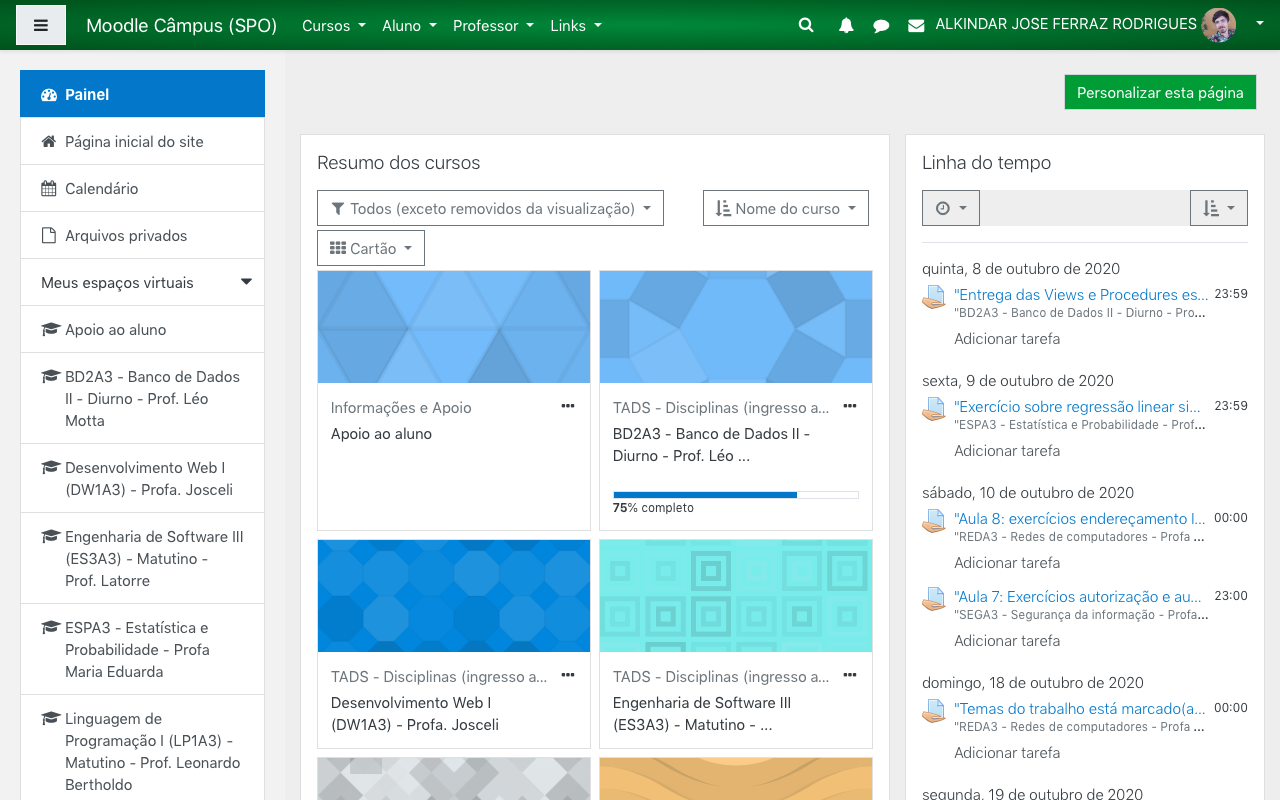
\includegraphics[width=.9\linewidth]{./media/painel.png}
\caption{\label{fig:orgd56bb7d}Painel de cursos do Moodle IFSP}
\end{figure}



\subsection*{Comentários de usuários sobre a inferface do Moodle IFSP}
\label{sec:org988a5ca}


\section*{Propstas de refatoração}
\label{sec:org9fed00b}

\section*{Wireframes}
\label{sec:org4cee4ac}

\section*{Conclusão}
\label{sec:org6b91cb5}
\end{document}
